\section{Эксперемент}

\begin{eqnarray}
    Al + CuSO_4 &\to& \emptyset \\  
    Al + CuCl_2 &\to& AlCl_2  + Cu  + E
\end{eqnarray}

В первом случае реакции не наблюдается, во втором случе рекция идет 
с очень большим выделением тепла.

\begin{equation}
    Al + CuSO_4 + NaCl + H_2O \to 
    AlCl_3 + 3H_2\uparrow + 3NaO + CuSO_4 \to  
    Al_2(SO_4)_3 + 3CuCl_2 + 3NaO
\end{equation}

\begin{figure}[h]
    \centering
    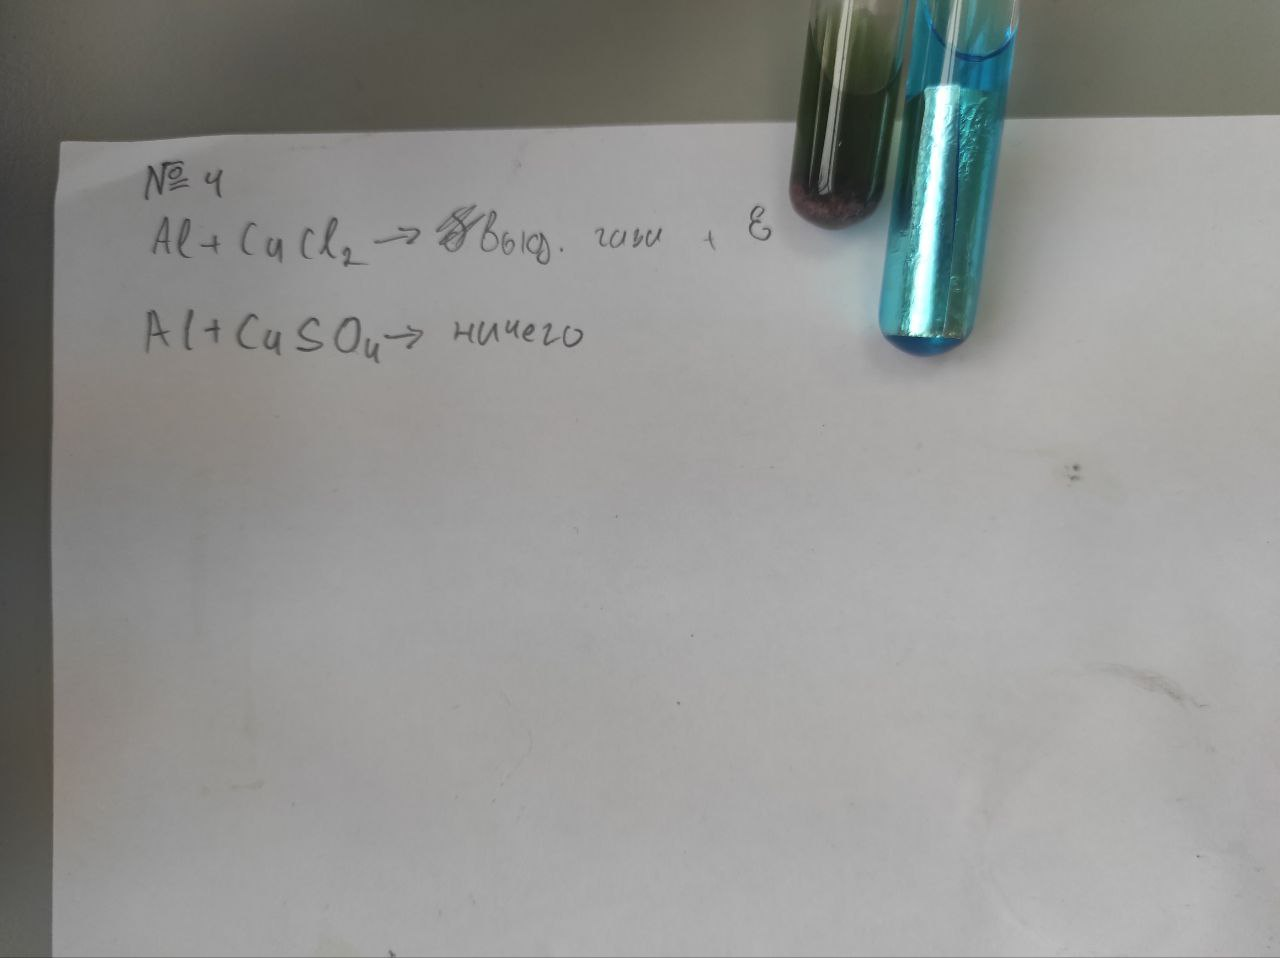
\includegraphics[trim={0 15cm 0 0},clip,width=\textwidth]{Ex_4/Ex_4_1.jpg}
     \caption{Результыты эксперемента}
    \label{Ex_4_1}
\end{figure}
\begin{figure}[h]
    \centering
    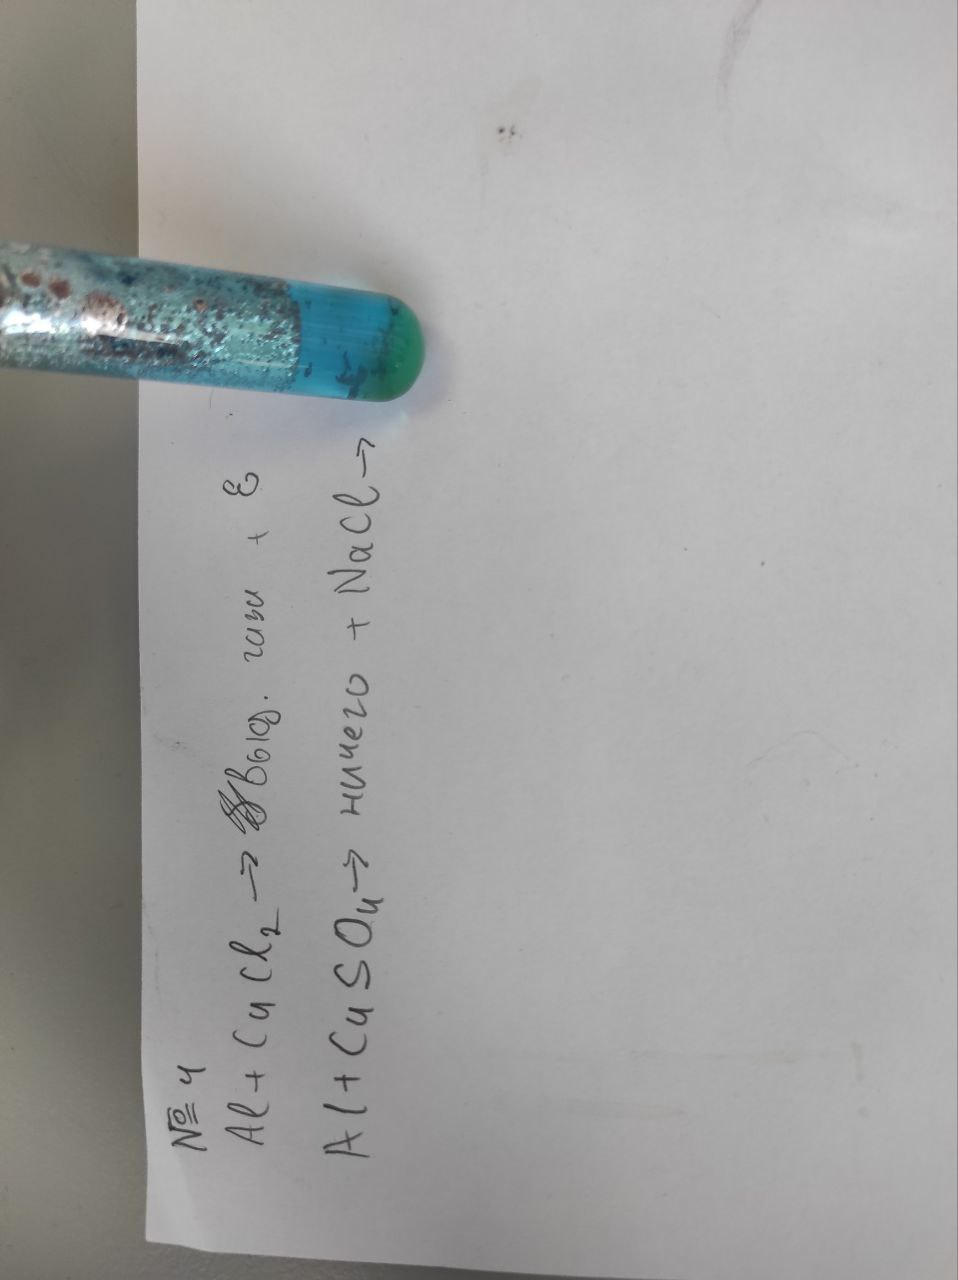
\includegraphics[trim={0 30cm 0 0},clip,width=\textwidth]{Ex_4/Ex_4_2.jpg}
     \caption{В пробирку с медным купоросом добавил хлорид меди}
    \label{Ex_4_2}
\end{figure}






